\documentclass[aspectratio=169,11pt]{beamer}

\usepackage[utf8]{inputenc}
\usepackage[T1]{fontenc}
\usepackage{booktabs}
\usepackage{graphicx}

\usetheme{Madrid}
\definecolor{accent}{RGB}{30,80,150}
\definecolor{good}{RGB}{30,120,70}
\definecolor{warn}{RGB}{160,60,40}
\setbeamercolor{structure}{fg=accent}
\setbeamercolor{frametitle}{bg=accent,fg=white}
\setbeamertemplate{navigation symbols}{}

\title{AgentIA}
\subtitle{Del dolor al estado actual: propuesta, auto-mejora, diseño, orquestación, interfaz y coste}
\author{Ingeniería AgentIA}
\date{2026-09-29}

\begin{document}

\begin{frame}
  \titlepage
\end{frame}

\begin{frame}{El dolor}
  \begin{block}{El problema}
    Generar un microservicio de producción es \textbf{caro, lento e inconsistente}.
    Cada servicio debe obedecer las mismas reglas --- capas estrictas, contratos
    inmutables, errores centralizados, compilación hermética --- y cada incumplimiento
    se paga en revisión, defectos o deuda técnica.
  \end{block}
  \begin{alertblock}{El síntoma}
    Durante meses la plataforma reportó \textbf{``0 de 15 sesiones verificadas''}:
    no podía demostrar que su propia salida compilaba.
  \end{alertblock}
  \begin{itemize}
    \item La causa era un defecto de montaje Docker de \textbf{un solo carácter}.
    \item Un sistema que no verifica su propia salida no puede prometer fiabilidad.
  \end{itemize}
\end{frame}

\begin{frame}{La propuesta}
  \textbf{Microservice Code Studio}: un agente autónomo que convierte una
  especificación formal en un microservicio Spring Boot \textbf{compilado y probado},
  y se niega a reportar éxito salvo que eso sea cierto.
  \begin{center}
    \begin{tabular}{ll}
      \toprule
      Entrada & especificación formal (blueprint + historias BDD) \\
      Generación & agente LangGraph de 8 etapas, gobernado por reglas \\
      Verificación & \texttt{mvn test -o} en Docker hermético (sin red) \\
      Reparación & acotada (máx.\ 3); al límite, \texttt{BLOQUEADO} $\rightarrow$ humano \\
      Entrega & ZIP o publicación Git atómica \\
      \bottomrule
    \end{tabular}
  \end{center}
  \textbf{La promesa no es ``código mejor'': es gobernanza, verificada y auditable.}
\end{frame}

\begin{frame}{La propuesta de auto-mejora}
  \begin{block}{El bucle reflexivo (construido, features 014--015)}
    Un LLM reflexiona sobre los \emph{diagnósticos} y propone ediciones a un documento
    de ``habilidad''; se admite una edición solo si su contribución medida es positiva,
    y se desaloja solo por debajo de un suelo de evidencia. Sin pesos, sin GPUs.
  \end{block}
  \begin{block}{La condición que lo gobierna}
    \emph{``Un bucle alimentado solo con un veredicto binario no es mejor que ningún
    bucle.''} (CoEvoSkills: 41.1 con oráculo opaco vs 42.4 sin evolución; 71.1 con
    verificador de diagnóstico.) Por eso se construyó primero el \textbf{canal de
    diagnóstico} y se aplazó el optimizador.
  \end{block}
  \begin{itemize}
    \item La polaridad (prohibiciones vs prescripciones) dio \textbf{nulo}; el
    \emph{contenido} de las instrucciones sí importa.
    \item Antes de auto-mejorar hay que hacer \textbf{determinista el verificador}.
  \end{itemize}
\end{frame}

\begin{frame}{Estado actual}
  \begin{itemize}
    \item \textbf{Primera compilación verificada} --- el defecto de montaje se corrigió;
    la plataforma ya verifica su salida.
    \item \textbf{Ambas rutas de producto verifican} --- la ruta secuencial antes
    generaba código sin compilarlo; hoy comparte la misma veta de verificación.
    \item \textbf{La métrica dejó de ser manipulable} --- de una densidad a una
    penalización absoluta relativa a una línea base congelada.
    \item \textbf{El verificador es intermitentemente inestable} ($\approx$33\%):
    4/6 bajo carga, 8/8 secuencial. Causa probable: reetiquetado SELinux \texttt{:Z}
    sobre una caché compartida. \emph{Es el siguiente punto a cerrar.}
  \end{itemize}
\end{frame}

\begin{frame}{El diseño guiado por especificación}
  \begin{center}
    \textbf{especificación $\rightarrow$ generación $\rightarrow$ verificación contra la especificación}
  \end{center}
  \begin{center}
    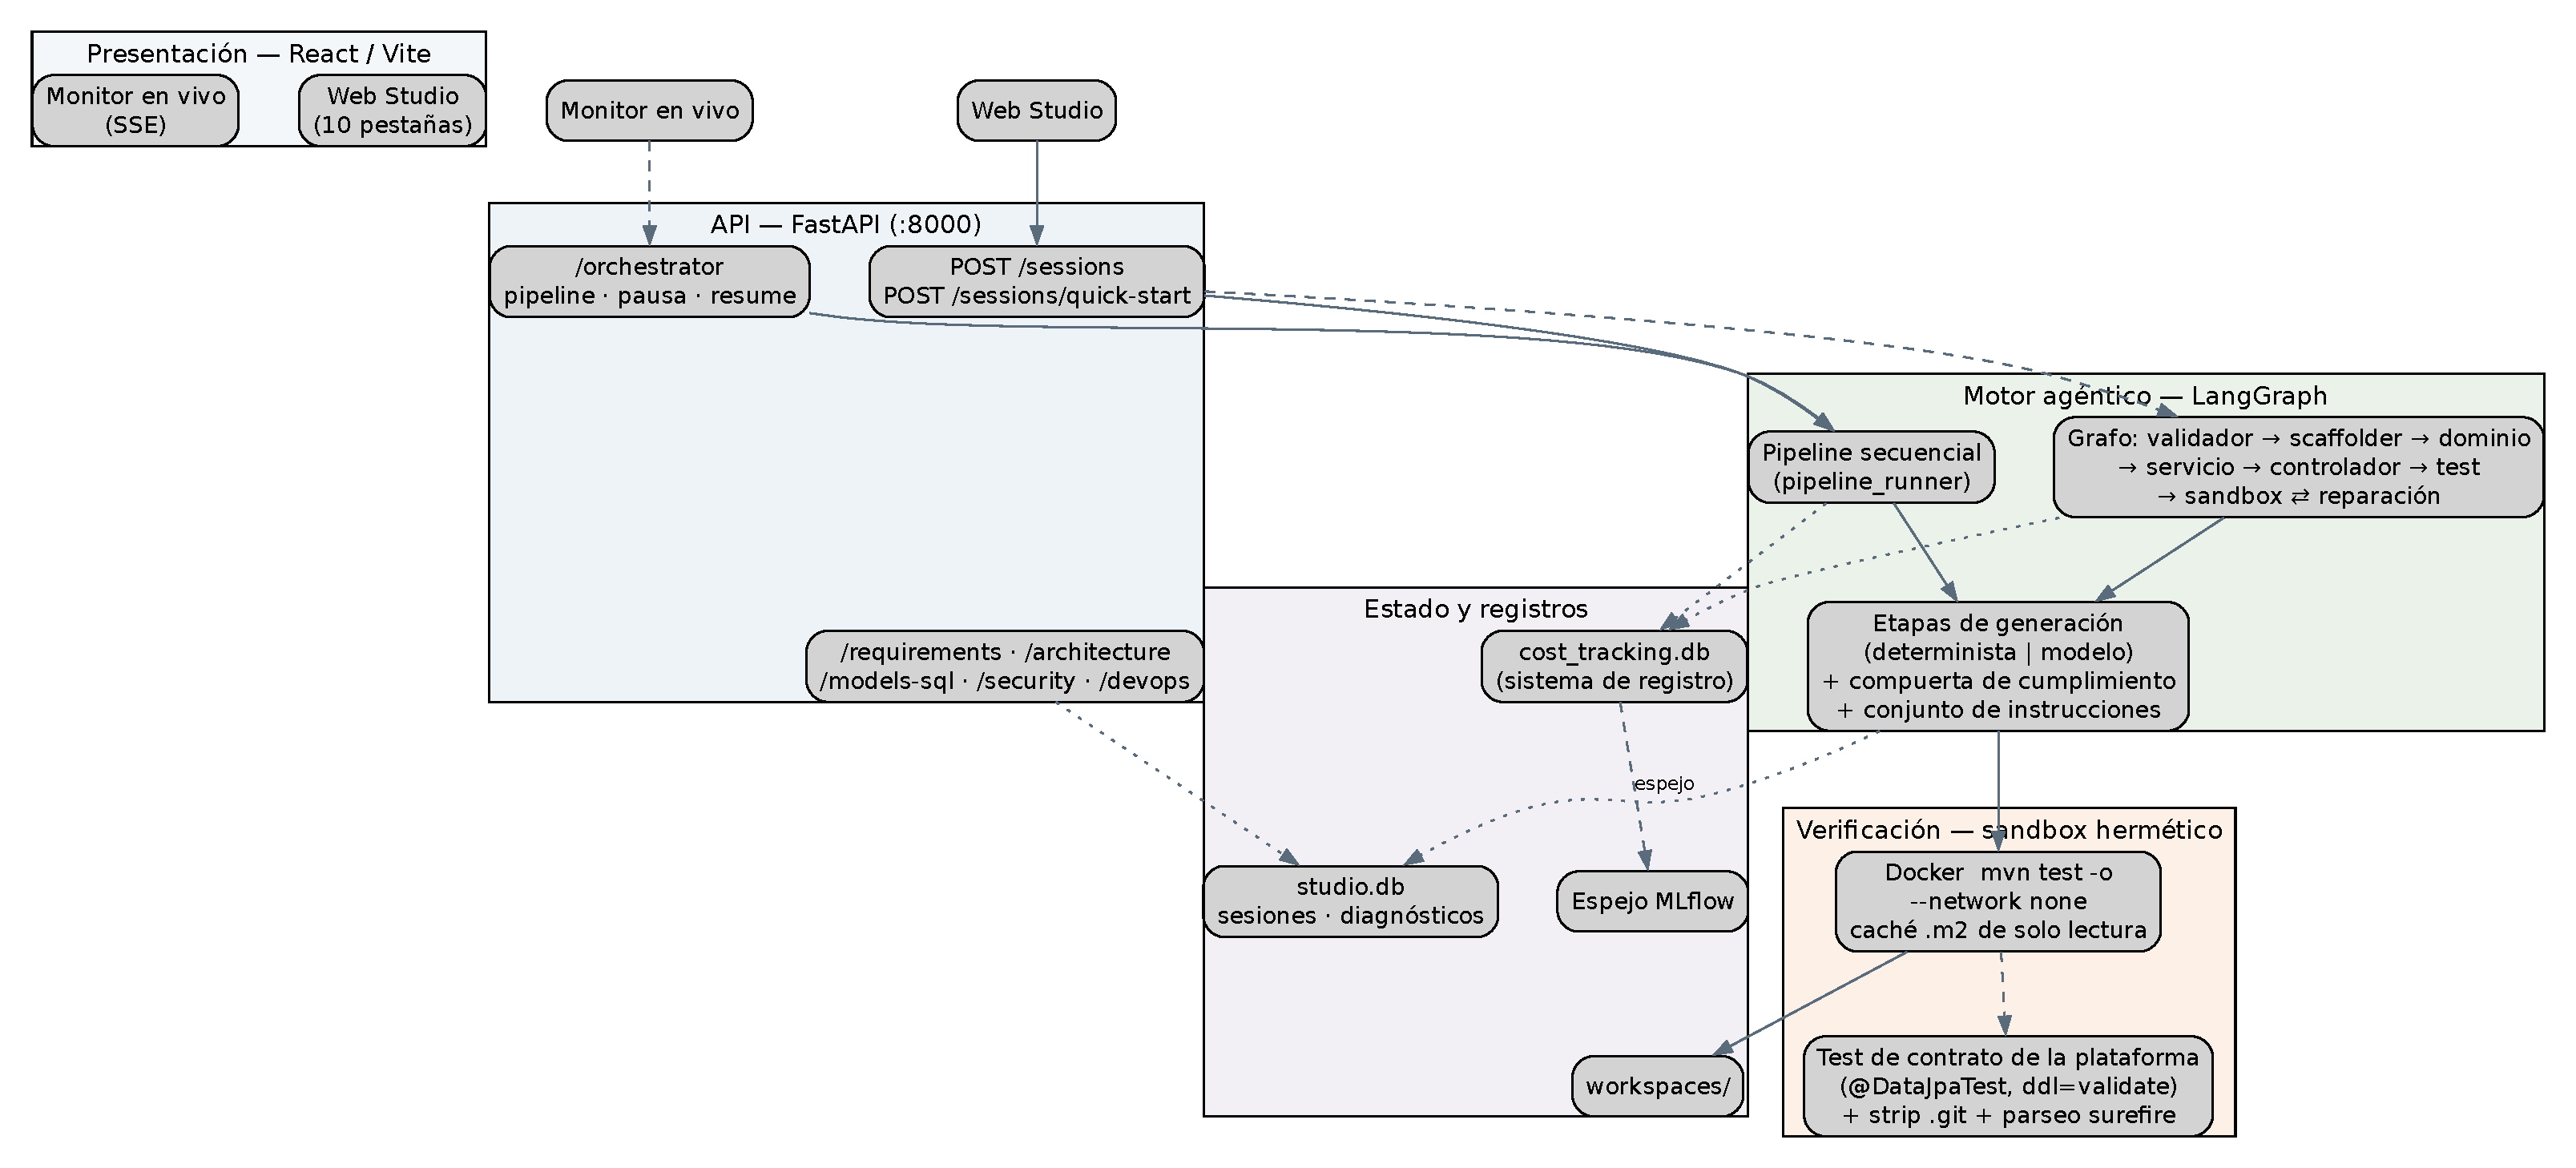
\includegraphics[width=0.98\textwidth]{fig/architecture.pdf}
  \end{center}
\end{frame}

\begin{frame}{El diseño guiado por especificación (2)}
  \begin{center}
    \begin{tabular}{p{0.40\textwidth}p{0.52\textwidth}}
      \toprule
      \textbf{Especificación} & \textbf{Qué prescribe} \\
      \midrule
      Blueprint / spec.md (Spec Kit) & entidades, validaciones, historias BDD, capas \\
      Constitución (6 principios) & capas, contratos inmutables, errores, offline, gates, secretos \\
      Documentos de instrucción (5) & el procedimiento por etapa \\
      Lista blanca de dependencias & el límite del pom.xml \\
      Contratos (19) & el comportamiento por feature \\
      \bottomrule
    \end{tabular}
  \end{center}
  \textbf{La especificación es la autoridad, no el modelo.}
\end{frame}

\begin{frame}{Orquestación de agentes y LangGraph}
  \begin{center}
    \texttt{validador $\rightarrow$ scaffolder $\rightarrow$ dominio $\rightarrow$ servicio
    $\rightarrow$ controlador $\rightarrow$ test $\rightarrow$ sandbox $\rightleftharpoons$ reparación}
  \end{center}
  \begin{center}
    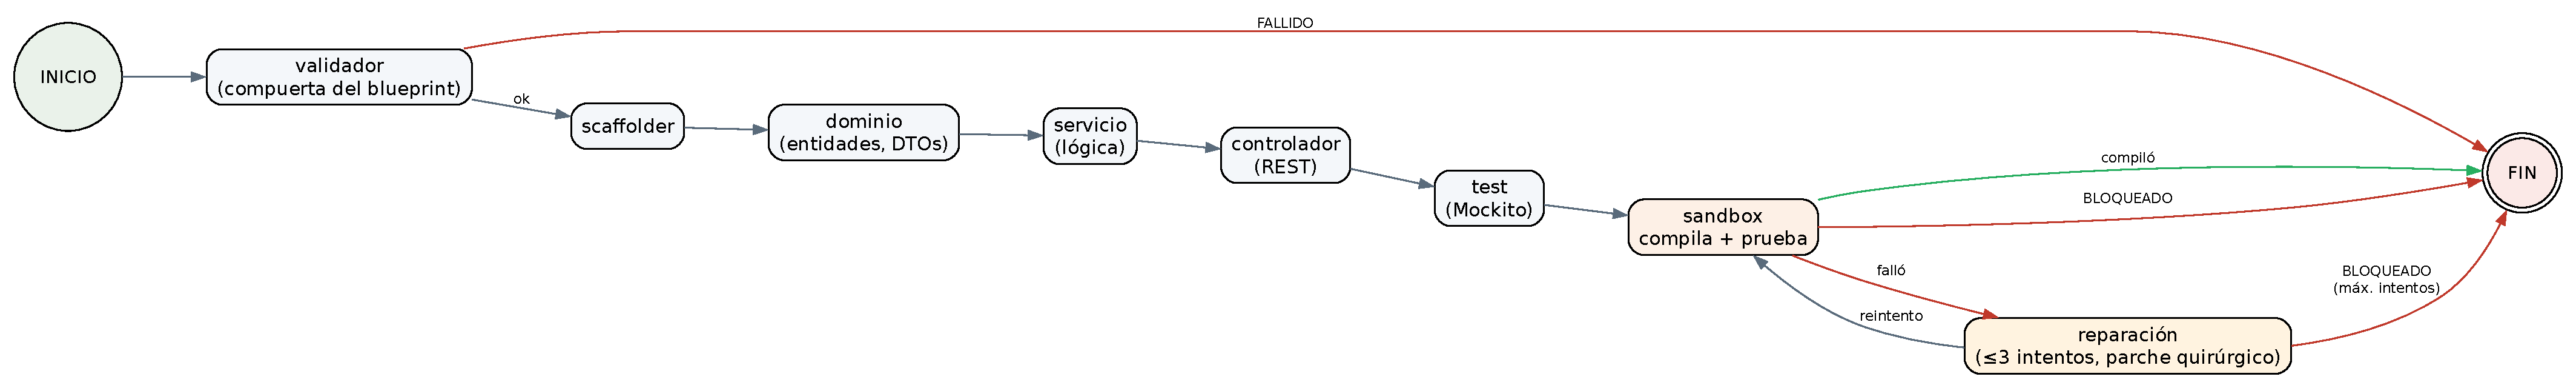
\includegraphics[width=0.72\textwidth]{fig/workflow.pdf}
  \end{center}
  8 agentes: 5 de modelo, 3 deterministas (validador, sandbox, reparación).
\end{frame}

\begin{frame}{Orquestación (2): qué se antepone a cada prompt}
  \begin{center}
    \begin{tabular}{p{0.52\textwidth}p{0.42\textwidth}}
      \toprule
      \textbf{Se antepone, en orden} & \textbf{Agente (pista del prompt)} \\
      \midrule
      prefijo de habilidad (hoy vacío) & \textbf{Scaffolder}: ``solo dependencias de la lista blanca'' \\
      documento de instrucción (system prompt) & \textbf{Dominio}: ``records nativos; \texttt{@Data} prohibido'' \\
      payload de la tarea (blueprint + previos) & \textbf{Servicio}: ``lógica solo en servicio; inyección por constructor'' \\
      rutas que posee & \textbf{Controlador}: ``un \texttt{@RestControllerAdvice} que registra la traza'' \\
      formato de respuesta (un JSON) & \textbf{Test}: ``cada escenario se mapea a un método'' \\
      \bottomrule
    \end{tabular}
  \end{center}
\end{frame}

\begin{frame}{El flujo de la aplicación}
  \begin{center}
    \begin{tabular}{p{0.34\textwidth}p{0.58\textwidth}}
      \toprule
      \textbf{Fase} & \textbf{Qué ocurre} \\
      \midrule
      1. Requisitos & historias BDD, exportación spec.md \\
      2. Arquitectura & componentes y contratos (Mermaid) \\
      3. Modelos \& SQL & entidades JPA, schema.sql, ER \\
      4. Blueprints & ingesta y validación spec.md / JSON \\
      5. Generación \& Monitor & síntesis + logs en vivo (SSE) \\
      6. Código \& Fix & explorador, diffs, desbloqueo manual \\
      7. Calidad SAST & auditoría, quality gate, remediación \\
      8. DevOps & Dockerfile, CI/CD, k8s, despliegue local \\
      9. Entrega & ZIP o Git atómico \\
      \bottomrule
    \end{tabular}
  \end{center}
\end{frame}

\begin{frame}{La interfaz de usuario}
  \begin{itemize}
    \item React/Vite de una sola página, \textbf{diez pestañas} en español.
    \item Tema \textbf{claro/oscuro}, stepper de ciclo de vida, visores \textbf{Mermaid}.
    \item Panel LLM: proveedor (Gemini, Groq, OpenAI, DeepSeek, mock), clave, modelo, verificación.
    \item Verificación honesta de tres estados; auditoría que eliminó resultados fabricados.
  \end{itemize}
  \begin{center}
    \begin{tabular}{p{0.46\textwidth}p{0.46\textwidth}}
      \toprule
      \textbf{A demostrar} & \textbf{Detalle} \\
      \midrule
      Pestaña 5 — Monitor Live & streaming SSE en vivo \\
      Pestañas 2--3 & diagramas Mermaid (arquitectura / ER) \\
      \bottomrule
    \end{tabular}
  \end{center}
\end{frame}

\begin{frame}{El coste}
  \begin{center}
    \begin{tabular}{lrrr}
      \toprule
      \textbf{Alcance} & \textbf{Llamadas} & \textbf{Coste (USD)} & \textbf{Tok. salida} \\
      \midrule
      Experimento de polaridad & 750 & 6.58 & --- \\
      Cinco congelados & 120 & 0.63 & --- \\
      Diez difíciles & 50 & 0.64 & --- \\
      Sondas / sueltas & $\approx$250 & $\approx$0.16 & --- \\
      \midrule
      \textbf{Total} & \textbf{1172} & \textbf{8.01} & \textbf{12.28M} \\
      \bottomrule
    \end{tabular}
  \end{center}
  \begin{itemize}
    \item \$0.052--\$0.077 por servicio; $\approx$\$0.005 por llamada; todo en \texttt{deepseek-flash}.
    \item Selección guiada por verificación: \textbf{\$0.20 por servicio fiable} (k=3).
  \end{itemize}
\end{frame}

\begin{frame}{El coste (2): el espejo MLflow}
  \begin{alertblock}{Se ha desviado (y puede verse vacío)}
    El espejo totaliza \textbf{\$6.39} frente a \textbf{\$8.01} (subestimación del 20\%).
    Además, \texttt{mlflow ui} abre el almacén vacío \texttt{mlruns/} en vez de
    \texttt{mlflow.db}, y los agregados de sesión (168) cayeron en el experimento
    legado \texttt{Default}, con 0 en \texttt{agentia}.
  \end{alertblock}
  \begin{itemize}
    \item Arrancar con \texttt{--backend-store-uri sqlite:///mlflow.db}.
    \item Reparar el targeting de experimento en \texttt{mlflow\_sink.py}.
  \end{itemize}
\end{frame}

\begin{frame}{Conclusión}
  \begin{block}{Dónde estamos}
    De ``no puede verificar su propia salida'' a ``genera, compila y verifica a
    \$0.06 por servicio'', con 100\% de cobertura con tres candidatos a \$0.20.
  \end{block}
  \begin{enumerate}
    \item Hacer \textbf{determinista el verificador} (un montaje).
    \item Hacer que la \textbf{medida pueda moverse} (minar fallos en reglas).
    \item Solo entonces, preguntar si un documento de habilidad aporta algo.
  \end{enumerate}
  El bucle de auto-mejora queda cerrado tras esa compuerta --- la misma que el diseño
  siempre exigió.
\end{frame}

\end{document}
